\fancyhead[LE]{\fontsize{8.5pt}{10pt}\selectfont\textbf{\textsf{\thepage}}\quad \textbf{\textsf{CHƯƠNG 1}}\quad \textsf{Các hàm số và Mô hình}}
\fancyhead[RO]{\fontsize{8.5pt}{10pt}\selectfont\textsf{MỤC 1.4}\quad \textsf{Hàm số mũ}\quad \textbf{\textsf{\thepage}}}

\noindent
\begin{minipage}[t]{0.265\textwidth}
    \fontsize{8pt}{10pt}\selectfont
    \vspace{3pt}
    \noindent Nếu $0 < b < 1$, thì $b^x$ tiến dần về $0$ khi $x$ tăng lên rất lớn. Nếu $b > 1$, thì $b^x$ tiến dần về $0$ khi $x$ giảm dần qua các giá trị âm. Trong cả hai trường hợp, trục $x$ là một tiệm cận ngang. Các vấn đề này sẽ được thảo luận trong Mục 2.6.

    \vspace{3pt}
    \begin{flushright}
        \textbf{\textsf{HÌNH 3}}
    \end{flushright}

    \vspace{3pt}
    \begin{flushright}
        \textbf{\textsf{HÌNH 4}}
    \end{flushright}

    \vspace{3pt}
    \begin{tcolorbox}[colback=black!4, colframe=black!15, arc=2mm, boxrule=0.5pt, left=4pt, right=4pt, top=4pt, bottom=4pt]
        \fontsize{7.5pt}{9.5pt}\selectfont
        \textbf{\textsf{www.StewartCalculus.com}}\\[2pt]
        Để ôn tập và thực hành sử dụng các Quy tắc của số mũ, hãy nhấp vào \textit{Review of Algebra}.
    \end{tcolorbox}

    \vspace{3pt}
    \noindent Để ôn tập về phép lấy đối xứng và tịnh tiến đồ thị, xem Mục 1.3.
\end{minipage}%
\hfill
\begin{minipage}[t]{0.708\textwidth}
    \fontsize{8.8pt}{11.5pt}\selectfont
    Đồ thị của các hàm số trong họ hàm số $y = b^x$ được thể hiện trong Hình 3 với nhiều giá trị khác nhau của cơ số $b$. Chú ý rằng tất cả các đồ thị này đều đi qua cùng một điểm $(0, 1)$ vì $b^0 = 1$ với $b \neq 0$. Đồng thời chú ý rằng khi cơ số $b$ càng lớn thì hàm số mũ tăng càng nhanh (với $x > 0$).

    \begin{center}
        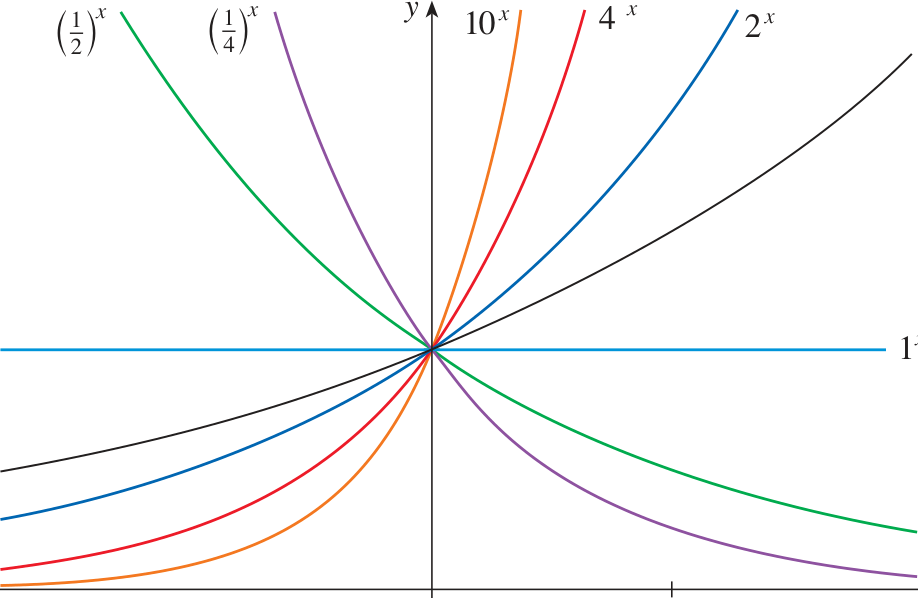
\includegraphics[width=0.64\linewidth]{images/p0082_fig3.png}
    \end{center}

    Từ Hình 3, bạn có thể thấy rằng về cơ bản có ba loại hàm số mũ $y = b^x$. Nếu $0 < b < 1$, hàm số mũ nghịch biến; nếu $b = 1$, nó là một hàm hằng; và nếu $b > 1$, nó đồng biến. Ba trường hợp này được minh họa trong Hình 4. Quan sát thấy rằng nếu $b \neq 1$, thì hàm số mũ $y = b^x$ có tập xác định là $\mathbb{R}$ và tập giá trị là $(0, \infty)$. Cũng lưu ý rằng, vì $(1/b)^x = 1/b^x = b^{-x}$, nên đồ thị của $y = (1/b)^x$ chỉ là phép lấy đối xứng qua trục $y$ của đồ thị hàm số $y = b^x$.

    \begin{center}
        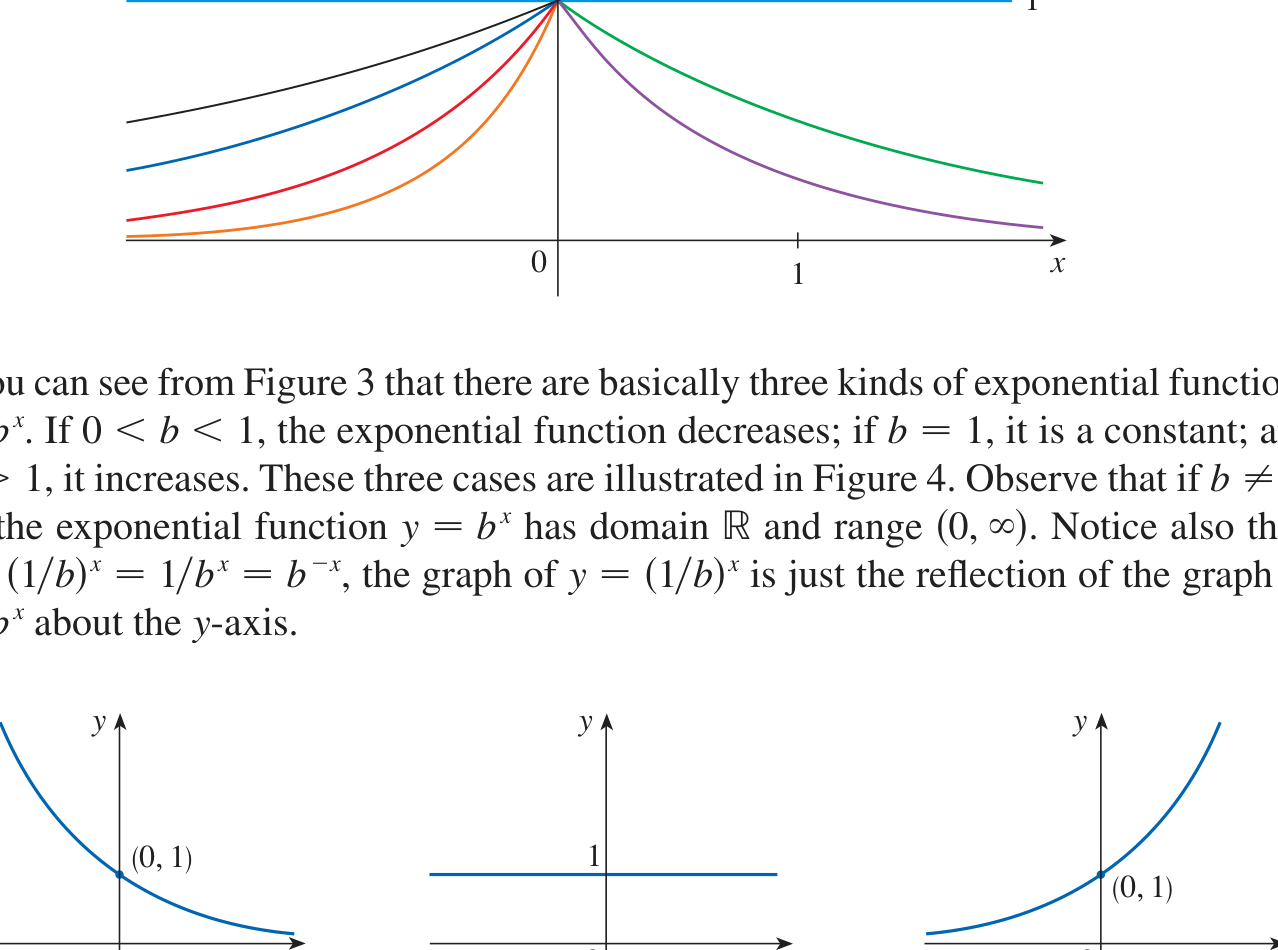
\includegraphics[width=0.66\linewidth]{images/p0082_fig4.png}
    \end{center}

    Một lý do cho tầm quan trọng của hàm số mũ nằm ở các tính chất sau đây. Nếu $x$ và $y$ là các số hữu tỉ, thì các quy tắc này đã rất quen thuộc từ đại số sơ cấp. Người ta có thể chứng minh rằng chúng vẫn đúng cho các số thực $x$ và $y$ tùy ý.

    \begin{definitionbox}
        {\bfseries\color{stewartred}Các quy tắc của số mũ}\quad Nếu $a$ và $b$ là các số dương và $x, y$ là các số thực bất kỳ, thì
        \vspace{3pt}
        
        \noindent
        \begin{tabular*}{\linewidth}{@{\extracolsep{\fill}}llll@{}}
            \textbf{1.} $b^{x+y} = b^x b^y$ & \textbf{2.} $b^{x-y} = \dfrac{b^x}{b^y}$ & \textbf{3.} $(b^x)^y = b^{xy}$ & \textbf{4.} $(ab)^x = a^x b^x$
        \end{tabular*}
    \end{definitionbox}

    \vspace{3pt}
    \noindent\textbf{\textsf{\color{stewartcyan}VÍ DỤ 1}}\quad Phác họa đồ thị của hàm số $y = 3 - 2^x$ và xác định tập xác định cùng tập giá trị của nó.

    \vspace{3pt}
    \noindent\textbf{\textsf{\color{stewartcyan}LỜI GIẢI}}\quad Trước tiên, ta lấy đối xứng đồ thị của $y = 2^x$ [được thể hiện trong các Hình 2 và 5(a)] qua trục $x$ để nhận được đồ thị của $y = -2^x$ trong Hình 5(b). Sau đó ta tịnh tiến đồ thị của $y = -2^x$
\end{minipage}